%% LaTeX Beamer presentation template (requires beamer package)
%% see http://bitbucket.org/rivanvx/beamer/wiki/Home
%% idea contributed by H. Turgut Uyar
%% template based on a template by Till Tantau
%% this template is still evolving - it might differ in future releases!

\documentclass{beamer}

\mode<presentation>
{
\usetheme{Warsaw}

\setbeamercovered{transparent}
%\setbeamercovered{dynamic}
}

\usepackage[english]{babel}
\usepackage[utf8]{inputenc}
\usepackage{graphicx}

\usepackage{booktabs}
\usepackage{hyperref}

%\usepackage[T1]{fontenc}

% More space between rows
\newcommand{\ra}[1]{\renewcommand{\arraystretch}{#1}}

\graphicspath{{./images/}}

%\setbeamertemplate{caption}[numbered]


% font definitions, try \usepackage{ae} instead of the following
% three lines if you don't like this look
\usepackage{mathptmx}
%\usepackage[scaled=1.0]{helvet}
%\usepackage{courier}

\setbeamertemplate{navigation symbols}{}
% \setbeamersize{text margin right=5pt}
\newenvironment{changemargin}[2]{% 
  \begin{list}{}{% 
    \setlength{\topsep}{0pt}% 
    \setlength{\leftmargin}{#1}% 
    \setlength{\rightmargin}{#2}% 
    \setlength{\listparindent}{\parindent}% 
    \setlength{\itemindent}{\parindent}% 
    \setlength{\parsep}{\parskip}% 
  }% 
  \item[]}{\end{list}} 

%\title{Playing with Stack Overflow data dump}
\title[The Wavelet Trie]{The Wavelet Trie: Maintaining an Indexed Sequence of
Strings in Compressed Space}

\subtitle{CSI 5335 Paper presentation}

% - Use the \inst{?} command only if the authors have different
%   affiliation.
%\author{F.~Author\inst{1} \and S.~Another\inst{2}}
\author[Roberto Grossi, Giuseppe Ottaviano]{{\bf Roberto Grossi, Giuseppe
Ottaviano}\\
presented by: Petr Praus}

\date{April 26th, 2012}


% This is only inserted into the PDF information catalog. Can be left
% out.
%\subject{Talks}



% If you have a file called "university-logo-filename.xxx", where xxx
% is a graphic format that can be processed by latex or pdflatex,
% resp., then you can add a logo as follows:

% \pgfdeclareimage[height=0.5cm]{university-logo}{university-logo-filename}
% \logo{\pgfuseimage{university-logo}}



% Delete this, if you do not want the table of contents to pop up at
% the beginning of each subsection:
%\AtBeginSubsection[]
%{
%\begin{frame}<beamer>
%\frametitle{Outline}
%\tableofcontents[currentsection,currentsubsection]
%\end{frame}
%}

% If you wish to uncover everything in a step-wise fashion, uncomment
% the following command:

%\beamerdefaultoverlayspecification{<+->}

\begin{document}

\begin{frame}
\titlepage
\end{frame}

\section{Use case}

\begin{frame}
\frametitle{Use case}
\begin{itemize}
  \item A lot of things are string sequences.
  \item Column databases store and index string sequences.
  \item Great example: access logs
\end{itemize}
\vspace{10pt}
{\scriptsize
188.26.52.117 - - [24/Apr/2013:03:35:48 -0500] "GET /img/welcome/corner.png\\
188.26.52.117 - - [24/Apr/2013:03:35:49 -0500] "GET /img/welcome/arrowDown.gif\\
188.26.52.117 - - [24/Apr/2013:03:35:49 -0500] "GET /img/welcome/regionals.jpg\\
}
\vspace{10pt}
\begin{changemargin}{-15pt}{-15pt}
\begin{itemize}
  \item Pretty similar, huh?
  \item I heard indexes make stuff faster $\rightarrow$ indexed sequence of strings
  \item Rank query: Number of requests for \texttt{/img/welcome/corner.png}?
  \item Select query: Position of $i$-th occurrence of \texttt{/img/welcome/corner.png}
\end{itemize}
\end{changemargin}
\end{frame}


\section{Building blocks}

\begin{frame}
\frametitle{Patricia Trie}
\begin{itemize}
  \item Space-efficient trie.
  \item Node has always has at least two children.
\end{itemize}
\begin{figure}
\scalebox{1.0}{\includegraphics{Patricia_trie.pdf}}
\end{figure}
\end{frame}


\begin{frame}
\frametitle{Wavelet Tree}
\begin{itemize}
  \item Organizes a string into a balanced binary tree of bit vectors.
  \item Alphabet: $\sum = \{a,b,c,d,r\} \rightarrow \{0, 0, 1, 1, 1\}$
  \item At root, we have \emph{ambiguity}, reducing ambiguity towards leaves
\end{itemize}
\begin{figure}
\scalebox{0.75}{\includegraphics{Wavelet_tree.png}}
\end{figure}
\end{frame}


\begin{frame}
\frametitle{Efficient computation of rank in Wavelet Tree}
\begin{itemize}
  \item $rank(8, a)$ = how many a's before position 8
  \item $rank_{bin}(pos, s)$ binary rank, \# of occurences of $s$ before $pos$  
\end{itemize}
\begin{figure}
\scalebox{0.6}{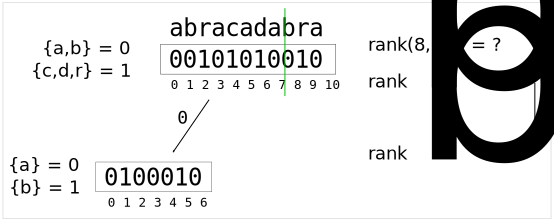
\includegraphics{wavelet_rank.pdf}}
\end{figure}
{\small E.g.: \# of requests to \texttt{/img/welcome/corner.png} before April 10th.}
\end{frame}


%\begin{frame}
%\frametitle{Outline}
%\tableofcontents
% You might wish to add the option [pausesections]
%\end{frame}

% \section{Data set}
% 
% \begin{frame}
% \frametitle{Data set}
% \begin{itemize}
%   \item Stack Exchange, Inc. periodically releasing dump of their data
%   \item Stack Overflow ($\approx$ 6GB), SuperUser, TeX, \ldots
%   \item Structured XML or custom-made Data Explorer
% \end{itemize}
% \begin{figure}
% \scalebox{.23}{\includegraphics{data_explorer}}
% \end{figure}
% \end{frame}
% 
% 
% \section{Prediction Task}
% %\subsection[Short First Subsection Name]{First Subsection Name}
% 
% \begin{frame}
% \frametitle{Tasks}
% \begin{block}{Asker Satisfaction Problem (related work)}
% Given a question submitted by an asker, predict whether the user will be
% satisfied with the answers contributed by the community.
% \end{block}
% \vspace{1em}
% \begin{itemize}
%   \item Lots of unanswered questions (50\% on Super User, 36\% SO)
%   \item First predict IF the question gets answered
%   \item Then predict WHEN the question gets answered
% \end{itemize}
% \begin{itemize}
%   \item Satisfactory answer = accepted answer
%   \item Good data (accepted answers, time, tags, post content, \ldots)
%   \item Surprisingly different tasks
% \end{itemize}
% \end{frame}
% 
% 
% \begin{frame}
% \frametitle{Techniques used}
% \begin{itemize}
%   \item Support Vector Machine for classification tasks
%   \item Support Vector Regression for regression tasks
%   \item Framework: Shogun Toolbox (Octave/Matlab, Python, \ldots)
%   \item Scaling ([0,1], SVM/Kernel can otherwise break)
%   \item Hold-out set for validation
% \end{itemize}
% \end{frame}
% 
% 
% %-------------------------------------------------------------------------------
% \section{Predicting IF the question gets answered}
% %-------------------------------------------------------------------------------
% 
% \begin{frame}
% \frametitle{IF Prediction}
% \framesubtitle{Will the question get answered at all?}
% \begin{itemize}
%   \item Binary classification problem
%   \item SVM is a go-to choice
%   \item Other options: kNN, Gaussian Naive Bayes
% \end{itemize}
% \vspace{1em}
% {\bf Selecting Features}
% \begin{itemize}
%   \item Asker's reputation, acceptance rate, and membership length
%   \item Visual quality of the question (Wh-words, \ldots)
%   \item Question tags
%   \item Question text body $\rightarrow$ NLP?
% \end{itemize}
% \end{frame}
% 
% 
% \begin{frame}
% \frametitle{IF Prediction: Validation Results - Super User}
% %\framesubtitle{}
% \begin{table}[t]
%     \centering
%     \ra{1.1}
%     \begin{tabular}{@{}lcc@{}} \toprule
%                      & Real positive & Real negative \\
%     \midrule
%     Predict positive & 1344           & 240 \\
%     Predict negative & 756           & 659 \\  
%     \bottomrule
%     \end{tabular}
%     %\caption{Number of edges matching ground truth}
%     %\label{t:edge_analysis}
% \end{table}
% \begin{itemize}
%   \item Super User data set (15000 randomly selected questions)
%   \item Test set: 2999 examples
%   \item 50 \% questions is unanswered!
%   \item Precision: 85\%
%   \item Recall: 64\%
%   \item Accuracy: 67\%
%   \item Features: Reputation, Acceptance Rate
%   \item ``Membership length'' makes things worse!
%   \item Results are better than predicting always True (baseline)
% \end{itemize}
% \end{frame}
% 
% 
% \begin{frame}
% \frametitle{IF Prediction: Visualization of SVM predictions}
% %\framesubtitle{}
% \begin{figure}
% \centering
% \scalebox{.5}{\includegraphics{svm_nice_separation}}
% %\caption{Visualization of SVM predictions}
% \end{figure}
% \begin{center}
% Red dot -- unanswered question, Green dot -- answered question
% \end{center}
% \end{frame}
% 
% 
% \begin{frame}
% \frametitle{IF Prediction: Validation Results - \TeX}
% %\framesubtitle{}
% \begin{table}[t]
%     \centering
%     \ra{1.1}
%     \begin{tabular}{@{}lcc@{}} \toprule
%                      & Real positive & Real negative \\
%     \midrule
%     Predict positive & 1838           & 184 \\
%     Predict negative & 369           & 188 \\  
%     \bottomrule
%     \end{tabular}
%     %\caption{Number of edges matching ground truth}
%     %\label{t:edge_analysis}
% \end{table}
% \begin{itemize}
%   \item TeX data set (12895 questions, 20\% withheld for validation)
%   \item Test set: 2579 examples
%   \item Precision: 92\%
%   \item Recall: 83\%
%   \item Accuracy: 79\%
%   \item Same features
%   \item Just 10 \% questions is unanswered
% \end{itemize}
% \end{frame}
% 
% 
% 
% 
% %-------------------------------------------------------------------------------
% \section{Predicting WHEN the question gets answered}
% %-------------------------------------------------------------------------------
% \begin{frame}
% \frametitle{WHEN Prediction}
% \framesubtitle{When we will get a satisfactory answer?}
% \begin{itemize}
%   \item Turns out to be much harder
%   \item Features should represent how appealing the question is to experts --
%   too hard
%   \item Notion of time might help
% \end{itemize}
% \begin{figure}
% \scalebox{.26}{\includegraphics{su-multiclass-scatter}}
% \end{figure}
% 
% \end{frame}
% 
% 
% \begin{frame}
% \frametitle{Time to answer vs. Time of day}
% \framesubtitle{How long it takes to answer a question depending on time of day}
% \begin{figure}
% \scalebox{.5}{\includegraphics{tex-answertime-timeofday}}
% \end{figure}
% \end{frame}
% 
% 
% \begin{frame}
% \frametitle{When are questions asked?}
% \begin{figure}
% \scalebox{.45}{\includegraphics{tex-hist-timeofday}}
% \end{figure}
% \end{frame}
% 
% 
% \begin{frame}
% \frametitle{WHEN Prediction: Validation Results - \TeX}
% \begin{itemize}
%   \item Same $\TeX$ data set
%   \item New feature: time of day (hour)
%   \item Median error: 22 minutes
%   \item Mean error: 51 minutes
%   \item Standard deviation of error: 68 minutes!
%   \item Way too much noise for something really accurate
% \end{itemize}
% {\bf Other features}
% \begin{itemize}
%   \item Question tags
%   \item Question text body $\rightarrow$ NLP?
% \end{itemize}
% \end{frame}
% 
% 
% 
% \begin{frame}
% \frametitle{Summary}
% \begin{itemize}
%   \item Freely available, up to date, large data set
%   \item Predicting IF the question gets answered is possible,\\
%         but only for sites with lay users
%   \item Meaningfully predicting WHEN the question gets answered is much harder,
%         data are extremely noisy
%   \item Possible approach to WHEN: track expert users and topics they answer
%   (some NLP needed) and match them with questions (again NLP)
%   \item \emph{Algorithm should be aware of question type.}  
% \end{itemize}
% \end{frame}


\begin{frame}
\frametitle{Summary}
\begin{center}
\large \bf Thank you.
\end{center}
\end{frame}
 
\begin{frame}
\frametitle{Resources}
\begin{itemize}
  \item \url{http://alexbowe.com/wavelet-trees/}
\end{itemize}
\end{frame}
 
 

%\begin{frame}
%\frametitle{}

% You can create overlays
% \begin{itemize}
%   \item using the \texttt{pause} command:
%   \begin{itemize}
%     \item First item.
%     \pause
%     \item Second item.
%   \end{itemize}
%   \item using overlay specifications:
%   \begin{itemize}
%     \item<3-> First item.
%     \item<4-> Second item.
%   \end{itemize}
%   \item using the general \texttt{uncover} command:
%   \begin{itemize}
%     \uncover<5->{\item First item.}
%     \uncover<6->{\item Second item.}
%   \end{itemize}
% \end{itemize}
% \end{frame}
% 
% \section*{Summary}
% 
% \begin{frame}
% \frametitle<presentation>{Summary}
% 
% \begin{itemize}
%   \item The \alert{first main message} of your talk in one or two lines.
% \end{itemize}
% 
% % The following outlook is optional.
% \vskip0pt plus.5fill
% \begin{itemize}
%   \item Outlook
%   \begin{itemize}
%     \item Something you haven't solved.
%     \item Something else you haven't solved.
%   \end{itemize}
% \end{itemize}
% \end{frame}
% 
% \end{document}
